\chapter{Mode Mapping}
\label{chap:mode_mapping}

\section{Pros and Cons of Existing Analysis}
\label{sec:mm:pros_n_cons}

\subsection{Pros}
\label{mm:pros}
Existing analysis has considered every possible delicate detail to compute the worst case execution time. Upsides of the analysis are discussed here.

\subsubsection{Cache Miss}
Memory access time is different for different memory hierarchy levels. For instance, register memory can be accessed in one cycle, L1 cache in few cycles, L2 cache in 10 cycles and local DRAM needs approximately 100 cycles to be accessed by the CPU. To compute magnitude square root of 20 elements and store back the results to L1 cache, a CPU requires 280 cycles if the data are in L1 cache, 2140 cycles if the data are in SDRAM, assuming 4 cycles L1 access time and 10 cycle execution time per element. This kind of major variations are unfavourable for determinism. One of the ways to calculate Worst Case Execution Time is to assume cache miss always. This is a pessimistic approach as the cache hit ratio is not always 0\%. 

\subsubsection{Memory Partitioning}
In time partition scheme, shared resources (L2 cache, Memory) are partitioned for A/A Mode and SAR Mode to provide segregation. This isolation clearly defines the accessible address space for each core. Even if SAR Mode processing of a core consumes huge memory space, A/A Mode data of the core remains intact and will be useful during next time slice. Another advantage of memory partitioning is load balancing. In Scheme-3 A/A Mode analysis, 81\% of the core4's L2 partition is utilized whilst only 6\% of the core1's L2 partition is utilized. This quantitative information helps to reconfigure the partition values to have good load balance.

\subsubsection{CPU Utilization Balancing}
In time partition scheme, CPU utilization factors for A/A Mode and SAR Mode can be well balanced by configuring time slot period. For instance, in space partition scheme, core4 is utilized 75\% in A/A Mode CPUs and 25\% in SAR Mode CPUs. This information gives a hint for time partitioning that A/A Mode needs more time span than SAR Mode in core4. It is adopted in Scheme-2, allocating 14.5ms for A/A Mode and 4.5ms for SAR Mode to balance the CPU utilization. Dynamic partition configuration can be considered in future to improve CPU load balancing.

\subsection{Cons}
\label{mm:cons}

\subsubsection{Context Switch Time}
Context switch time of 0.5ms is assumed for time partitioning. Every core does 2 context switches in 20ms. In time partition analysis (Scheme2 and Scheme3), at the end of 19.50ms all the four cores want to perform context switching. Since the SDRAM has only one port, it is possible for only one core to access the memory. Other cores have to wait till that time. 

\begin{figure}[h!]
	\centering
	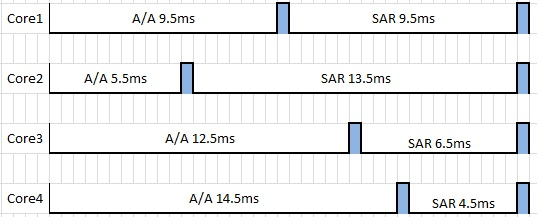
\includegraphics[width=120mm]{figures/mm_cons1}
	\caption{Time Partition of Scheme 3}
	\label{fig:mm:mm_cons1}
\end{figure}

Assuming the order of SDRAM access is core1, core2, core3 and core4. Core2 waits for core1 to complete (0.5ms), core3 waits for core1,2 (0.5ms + 0.5ms), core4 waits for core1,2,3 (0.5ms + 0.5ms + 0.5ms). This overhead in waiting time sums up to 3ms. Though only one context switch is contending, during the course of run it will be a scenario where two context switches will contend for SDRAM because of its skewed timing behaviour. Worstcase waiting time for four cores is 
	\begin{equation}
		\begin{split}
			& = \frac{4*ContextSwitchTime \enspace + \enspace 2*OverheadInWaitingTime}{AvailableTime} \\[0.4cm]
			& = \frac{4*2*0.5ms \enspace + \enspace 2*3ms}{4*20ms}
			  = 12.5\%
		\end{split}
	\end{equation}

In the worst case scenario, 12.5\% of the CPU time is spent only for context switching. This percentage is severe for a Radar processor. It degrades the application performance and much meaningful processing can be done during that time. \\

\textbf{\textsl{Verification:}} LMbench microbenchmark\cite{lmbench} is used to measure the context switch time of the ARM cores. Different sets of processes and data size are examined for the context switch time measurement. 2p/16K in Table \ref{mm:ctxsw:lmbench} means that 2 processes, having working data set of 16KiB memory each are involved in context switch.

\begin{table}[h!]
	\begin{tabularx}{\textwidth}{|*{8}{Y|}}
		\hline
		\multirow{2}{*}{\textbf{\#Run}} & \multicolumn{7}{c|}{\textbf{Context Switch Time[\boldmath$\mu$s]}} \\ \cline{2-8}
		& \textbf{2p/0K} & \textbf{2p/16K} & \textbf{8p/16K} & \textbf{16p/16K} & \textbf{2p/64K}  & \textbf{8p/64K} & \textbf{16p/64K} \\ \hline 
		1 & 4.7 & 18.2 & 45.0 & 45.6 & 8.14  & 156.6 & 222.3 \\ \hline
		2 &  0.670 & 18.2 & 44.5 & 45.9 & 5.70 & 208.9  & 280.1 \\ \hline
		3 & 0.610 & 28.9 & 44.4 & 48.0 & 14.0 & 82.0 & 175.9 \\ \hline
	\end{tabularx}
\caption{Measured Context Switch Time}
\label{mm:ctxsw:lmbench}
\end{table}

\begin{figure}[h!]
\centering
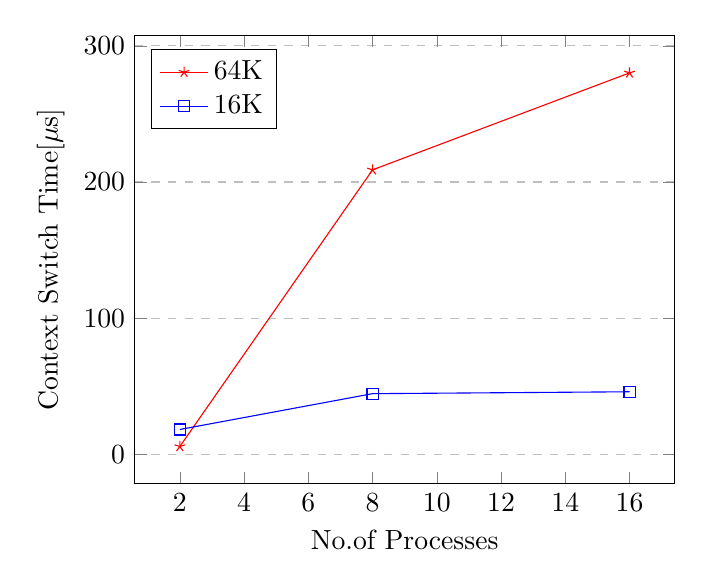
\begin{tikzpicture}
\begin{axis}[
	xlabel={No.of Processes},
	ylabel={Context Switch Time[$\mu$s]},
	legend pos=north west,
	ymajorgrids=true,
	grid style=dashed,
]
\addplot[color=red, mark=star,]
	coordinates {
		(2, 5.70) (8, 208.9) (16, 280.1)
	};

\addplot[color=blue, mark=square,]
	coordinates {
		(2, 18.2) (8, 44.5) (16, 45.9)
	};

	\legend{64K, 16K}
\end{axis}
\end{tikzpicture}
\caption{Comparison of Context Switch Time}
\label{mm:cntxt_switch_graph}
\end{figure}

From the above three sets of measurements, worst-case context switch time is 280$\mu$s corresponds to the 16 processes operating on 64KiB memory size. Also it reveals that the context switch time is proportional to the number of processes, as well as the data set size. On contrary to the assumption of 0.5ms context switch time and 12.5\% degradation in CPU utilization, measured worst-case context switch time is much lesser, therefore will not deteriorate the CPU utilization.

\subsubsection{Clashing Data Streams}
In time partition scheme, assume that a core is executing A/A Mode time slice. Now, SAR Mode data is routed to the same core by PSM2. The core cannot accept the SAR Mode data as it is executing A/A time slice and the PSM have no idea of what the cores are up to or what to do with the data if the core is not accepting. This corner case is not clearly defined in the existing analysis, as a result it leads to data loss if no countermeasure is provided. \\[0.2cm]
One of the ways to resolve this is to have a buffer in PSM to store the incoming data stream. If the core is not accepting the data, corresponding \verb|core_id| and \verb|cpu_id| shall be stored in PSM along with the data. When the core is requesting data during next SAR Mode time slice, the PSM can transfer the stored data if the \verb|core_id| and \verb|cpu_id| matches. Since the incoming data stream is stored for one time slice period, it has to be counted for the processing latency calculation. The storing and restoring scheme ensures that the A/A data and SAR data will never be routed to the same CPU at the same time. Applying this strategy to the Scheme-2 avoids both the data streams meeting at the same point, therefore the interfaces will not be as over utilized as 120\%. In effect, the peak interface utilization will be maximum of A/A Mode utilization(72.35\%) and SAR Mode utilization(48.01\%) resulting 72.35\%.

\subsubsection{Scalability}
\label{sss:mm:cons:scalability}
For time slot adjustment, it is cumbersome task to break the entire application in to pieces such that each and every piece will fit in to one time slot. Whenever there is a change in time slot period, the entire application requires rework to suspend itself before the time slot expires. It implies that the time and cost of the application development, maintenance will soar up in the sky. This doesn't stop here, amendments are needed if the Radar configuration such as PRF set is changed.


\subsection{Other Comments}
\subsubsection{Interface Utilization}
The peak interface utilization of Scheme-3 A/A Mode analysis is calculated as 78.93\% (see Chapter \ref{sss:scheme3:aa_interface_util}), considering only the input data rate. However, CPU input interface can never be utilized more than the input data rate which is 72.31\%. To put it in other words, peak interface utilization is nothing but the peak data rate as long as there is no interference in communication. 

\subsubsection{Typo}
Decimal conversion format(1000 Byte = 1KB) was used for byte conversion. This is changed to Binary conversion format (1024 Byte = 1KiB) to comply the standards. It has significant impact in the analysis results. An example is shown for interface utilization calculation of Scheme-1 in Chapter \ref{sec:scheme1:aa_interface_util}.

\begin{align*}
	\label{equ:mm:typo}
	iCON1 \: output \: to \: PSM1 &= \#\frac{byte}{sample} * \#channel * range \: gate * frequency \\
	&= 4 * 9 * 103 * 19.5kHz = 72306000 \frac{byte}{sec} = 72.3 \: MB/s \\
	Actual \: data \: rate &= \frac{72306000}{1024 * 1024} = 69 \: MiB/s \stepcounter{equation}\tag{\theequation}
\end{align*}

\subsubsection{Ideal Data Set Size}
Benchmarked functions have ideal data set range. For instance, matrix size of [1000 x 8] elements is processed to measure the execution time of complex multiply(CMY) function. Assuming 4 byte for a complex sample, 128-bit advanced SIMD unit(NEON) can hold four elements of CMYACC in a Q register and four multiplier elements in another Q register. Results of four multiplications are computed at the cost of one multiplication operation. But in reality, size of the data set is not always multiple of 128-bit. To compute CMY of [1000 x 9] data set, first eight elements of a row can be multiplied in SIMD lanes, last one element can be processed as normal multiplication operation. By doing so, it requires same execution time to process [1000 x 9] data set and [1000 x 12] data set, neglecting intrinsic load-store time. This performance constraint has to be taken into account for the full-fledged application development.

\subsubsection{OS overhead}
Operating system overhead of 1.3 was included in the analysis. As the execution time are measured in \verb|Linaro| OS, redundant \textsl{OSoverhead} factor is removed for further analysis.

\subsubsection{Execution Cycle Mismatch}
\label{mm:cons:exe_cyl_mismatch}
Execution cycle reported in Chapter \ref{tbl:aa_exe} and the measured execution cycle of the benchmark functions do not match. The reported values are much lower than the actual measured values. These values are amended according to the measured values for Mode Mapping analysis. Table \ref{tbl:mm:aa_real_exe_cycle} gives the comparison of old values versus new values for A/A Mode benchmarks.

\begin{table}[h!]
	\centering
	\begin{tabular}{|l|l|l|} 
	 \hline
	 \textbf{Benchmark} & \textbf{Old value [cycles]} & \textbf{Measured value [cycles]} \\
	 \hline
	 CMYACC8 & 79 & 287 \\ \hline
	 RMY50 & 15 & 68 \\ \hline
	 CONV128 & 24100 & 27300 \\ \hline
	 COT50 & 12 & 98 \\ \hline
	 FFT256 & 29700 & 37490 \\ \hline
	 MAG256 & 20 & 41 \\ \hline
	 AVG256 & 20 & 51 \\ \hline
	 CMPR256 & 7 & 55 \\ \hline
	 DET256 & 10 & 97 \\ \hline
	\end{tabular}
	\caption{Comparison of Old Execution Cycle vs Measured Execution Cycle of A/A Mode Benchmarks}
	\label{tbl:mm:aa_real_exe_cycle}
\end{table}

\FloatBarrier
\subsection{Measured Values of Existing Analysis}
\label{mm:cons:real_values}

The following latency and CPU utilization values are obtained for Existing Analysis, after updating the execution cycle values and removing OS overhead factor.

\subsubsection{Scheme-1}
\begin{table}[h!]
	\centering
	\begin{tabular}{|c|l|l|l|} 
	 \hline
	 \textbf{Look direction} & \textbf{Dwell time[ms]} & \textbf{Latency[ms]} & \textbf{\#Dwell latency} \\
	 \hline
	 1 & 27.84 & 416.40 & 14.96 \\ \hline
	 2 & 33.07 & 482.28 & 14.58 \\ \hline
	 3 & 39.17 & 574.52 & 14.67 \\ \hline
	 4 & 46.20 & 662.80 & 14.35 \\ \hline
	 5 & 54.26 & 798.62 & 14.72 \\ \hline
	\end{tabular}
	\caption{Measured Processing Latency of Scheme-1, A/A Mode}
	\label{tbl:mm:scheme1_true_latency}
\end{table}

\begin{table}[h!]
	\centering
	\begin{tabular}{|l|l|l|l|l|} 
	 \hline
	& \textbf{Core1} & \textbf{Core2} & \textbf{Core3} & \textbf{Core4} \\ \hline
	\textbf{Utilization} & 19.03\% & 46.20\% & 65.78\% & {\color{red} 108.07\%} \\ \hline
	\end{tabular}
	\caption{Measured CPU Utilization of Scheme-1, A/A Mode}
	\label{tbl:mm:scheme1_true_util}
\end{table}

\subsubsection{Scheme-2}
\begin{table}[h!]
	\centering
	\begin{tabular}{|l|l|l|l|l|} 
	 \hline
	& \textbf{Core1} & \textbf{Core2} & \textbf{Core3} & \textbf{Core4} \\ \hline
	\textbf{Utilization} & 25.00\% & {\color{red} 103.33\%} & 71.43\% & 83.33\% \\ \hline
	\end{tabular}
	\caption{Measured CPU Utilization of Scheme-2, A/A Mode}
	\label{tbl:mm:scheme2_true_util}
\end{table}

\begin{table}[h!]
	\centering
	\begin{tabular}{|c|l|l|l|} 
	 \hline
	 \textbf{Look direction} & \textbf{Dwell time[ms]} & \textbf{Latency[ms]} & \textbf{\#Dwell latency} \\
	 \hline
	 1 & 27.84 & 860.00 & 30.89 \\ \hline
	 2 & 33.07 & 920.00 & 27.82 \\ \hline
	 3 & 39.17 & 1060.00 & 27.06 \\ \hline
	 4 & 46.20 & 1220.00 & 26.41 \\ \hline
	 5 & 54.26 & 1520.00 & 28.01 \\ \hline
	\end{tabular}
	\caption{Measured Processing Latency of Scheme-2, A/A Mode}
	\label{tbl:mm:scheme2_true_latency}
\end{table}

\FloatBarrier
\subsubsection{Scheme-3}
\begin{table}[h!]
	\centering
	\begin{tabular}{|c|l|l|l|} 
	 \hline
	 \textbf{Look direction} & \textbf{Dwell time[ms]} & \textbf{Latency[ms]} & \textbf{\#Dwell latency} \\
	 \hline
	 1 & 27.84 & 920.00 & 33.05 \\ \hline
	 2 & 33.07 & 1060.00 & 32.05 \\ \hline
	 3 & 39.17 & 1220.00 & 31.15 \\ \hline
	 4 & 46.20 & 1380.00 & 29.87 \\ \hline
	 5 & 54.26 & 1680.00 & 30.96 \\ \hline
	\end{tabular}
	\caption{Measured Processing Latency of Scheme-3, A/A Mode}
	\label{tbl:mm:scheme3_true_latency}
\end{table}

\begin{table}[h!]
	\centering
	\begin{tabular}{|l|l|l|l|l|} 
	 \hline
	& \textbf{Core1} & \textbf{Core2} & \textbf{Core3} & \textbf{Core4} \\ \hline
	\textbf{Utilization} & 23.33\% & {\color{red} 103.33\%} & 63.33\% & 90\% \\ \hline
	\end{tabular}
	\caption{Measured CPU Utilization of Scheme-3, A/A Mode}
	\label{tbl:mm:scheme3_true_util}
\end{table}
\FloatBarrier

\subsubsection{Inference}
The Existing Analysis will not meet real-time requirements as the CPU cores are utilized more than 100\%. Another down side is the 15x dwell latency, which is not in the acceptable range.
%%%%%%%%%%%%%%%%%%%%%%%%%%%%%%%%%%%%%
%%%%%%%%%%%%%%%%%%%%%%%%%%%%%%%%%%%%%
%%%%%%%%%%%%   SECTION   %%%%%%%%%%%%
%%%%%%%%%%%%%%%%%%%%%%%%%%%%%%%%%%%%%
%%%%%%%%%%%%%%%%%%%%%%%%%%%%%%%%%%%%%
\section{Test Procedure} 
\label{sec:mm:test_procedure}
Executable code is transferred to the Nitrogen6X board via Ethernet. Benchmark profiling are done as follows.

%%%%%%%%%%%%%%%%%%%%%%%%%
%%%%%   SUB-SECTION   %%%
%%%%%%%%%%%%%%%%%%%%%%%%%
\subsection{Memory Transfer Bandwidth}
\label{ss:mm:mem_bw}
STREAM benchmark\cite{McCalpin2007} is used to measure memory bandwidth of the machine. The STREAM benchmark is a simple, synthetic benchmark designed to measure sustainable memory bandwidth (in MB/s) and a corresponding computation rate for four simple vector kernels namely Copy, Scale, Add and Triad \cite{streamDef}. Peak achievable memory bandwidth is measured by running threaded STREAM benchmark on Nitrogen6X board. Only STREAM benchmark is started by the user to guarantee that the measurement is not affected by other user applications.  STREAM benchmark is compiled and executed as follows: \\

\lstset{ %
  backgroundcolor=\color{grey},
  numbers=left,
  numberstyle=\tiny\color{mygray},
  frame=single,
  showspaces=false,
  showstringspaces=false,
  basicstyle=\ttfamily,
}

\begin{lstlisting}
user$ gcc -fopenmp -D_OPENMP stream.c -o stream
user$ export OMP_NUM_THREADS=4
user$ ./stream
\end{lstlisting}

The measurement result of copying data from one memory location to another memory location is used for the  analysis. To measure the peak data transfer rate, the best result from 5 consecutive run is computed. It is turned out that the iMX6Quad is capable of transferring \textbf{1048 MiB/s} when all the four cores are running in parallel.\\

\begin{table}[h!]
	\centering
	\begin{tabular}{|l|l|l|l|l|} 
	 \hline
	 \textbf{Function} & \textbf{Best Rate [MB/s]} & \textbf{Avg time[s]} & \textbf{Min time[s]} & \textbf{Max time[s]} \\
	 \hline
	 Copy & 1048.7 & 0.177625 & 0.152575 & 0.217059 \\ \hline
	\end{tabular}
	\caption{Idle Memory Transfer Bandwidth}
	\label{tbl:mm:bw_no_load}
\end{table}

To compute the peak memory bandwidth of the Radar application, STREAM benchmark is allowed to run in background along with the Radar application. STREAM is given low priority to give precedence to the Radar application. When the Radar application is consuming maximum bandwidth, STREAM can only consume the minimum leftover bandwidth. Subtracting minimum recorded bandwidth from the peak memory bandwidth of the iMX6Quad (1048 MiB/s), gives peak memory bandwidth utilized by the Radar application. Command for running STREAM benchmark at low priority: \\
\begin{lstlisting}
user$ sudo nice -n 19 ./stream >> ${OUTPUT_FILE}
\end{lstlisting}

%%%%%%%%%%%%%%%%%%%%%%%%%
%%%%%   SUB-SECTION   %%%
%%%%%%%%%%%%%%%%%%%%%%%%%
\subsection{Peak Memory Utilization}
\label{ss:mm:mem_util}
The percentage of the memory being used by a process can be extracted from \bverb|top| command. A bash script is written to read memory utilization 10 times a second (Appendix \ref{app:code:mem_util}) until the Radar application is running. Peak Memory Utilization is exported to an output file for further analysis. This script is also run in background at low priority along with the Radar application as follows.\\
\begin{lstlisting}
user$ sudo nice -n 19 ./mem_util.sh &
\end{lstlisting}

%%%%%%%%%%%%%%%%%%%%%%%%%
%%%%%   SUB-SECTION   %%%
%%%%%%%%%%%%%%%%%%%%%%%%%
\subsection{Latency (Worst Case Execution time)}
\label{ss:mm:latency}
Proper way of measuring the worst case execution time includes the following steps:
\begin{compactitem} 
	\item All the cores are set to begin the execution simultaneously to produce maximum contention.
	\item Cache data are invalidated before and after the measurement to ensure that the data is fetched from memory.
\end{compactitem} 

\noindent
The following methods are followed to improve the determinisism:
\begin{compactitem} 
	\item Cores are running fixed block of code(thread), 
	\item Radar application is given higher priority than other user space programs. \\
\end{compactitem} 

In worst case scenario, all the four cores will execute the same benchmark, generating L2 cache and memory contention. To ensure that all the cores are executing the same benchmark, \bverb|wait_for_all_threads()| function is provided (Appendix \ref{app:code:wait_for_others}). A thread reaches this function will wait for all the other threads to join. \\

Invalidating cache data from user space is not allowed in ARM Cortex A9 processor. On the other hand, writing a program that copies huge junk of data from one memory location to other memory location seems to clear the cache contents. But, because of the complex caching strategies, it is not guaranteed that the entire cache data are removed, thus leaving major portion of the cache intact.\footnote{A discussion about this in ARM Connected Community forum can be found at \url{http://community.arm.com/thread/8799}} 

To overcome this, the Radar benchmark sequences are executed for 1000 iterations to measure the maximum execution time. A graph is drawn on the iteration data. However, there are some unexpected spikes ranging 5 times higher than the average execution time. They are occurring at sporadic intervals. The Nitrogen6X board is running \verb|ssh, GUI,| \\ \verb|network-manager|, background tasks for measurement and other OS applications along with the benchmark application. It can be reasoned that any of the other applications interrupts a running thread, causing it to be blocked for a while. So, the measurement is showing unrealistic values.

\begin{figure}[h!]
	\centering
	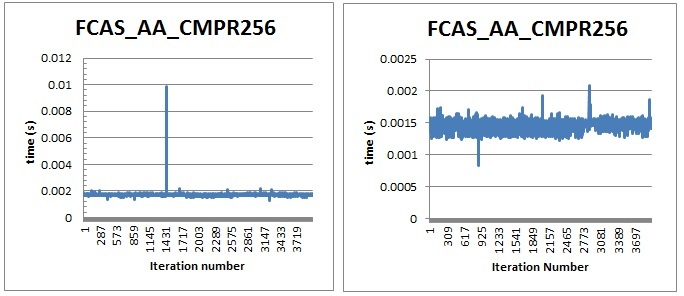
\includegraphics[width=150mm]{figures/chop_off}
	\caption{Before and After Spike Removal}
	\label{fig:mm:chop_off}
\end{figure}
A test run is made to study the effect of background tasks and services on the spikes. The background measurement tasks and services other than \verb|ssh, network-manager| are stopped. Now, only the minimal OS services are running. The Radar application is allowed to run in such less competitive environment. The result shows that the spikes are still occurring in few benchmarks, but the magnitude has reduced to 2x from 5x. As expected, some benchmarks do not have the spikes at all. It is concluded that the OS applications or services might have pre-empted the Radar application. Those spikes are removed from the graph and then the maximum execution time is computed. \vspace*{0.2cm}

To effectively utilize all the available four cores, four threads are spawned from main thread to carry out the parallel execution. Core affinity of each thread is set such a way that four threads are mapped to four cores (Appendix \ref{app:code:core_affinity}). For example, thread0 will run on core0, thread1 on core1, thread2 on core2 and thread3 on core3. \\

The Radar application is given higher priority than other user space tasks to give precedence. The following command is issued on Linaro Linux. 
\begin{lstlisting}
user$ sudo nice -n -20 ./AA_space_opt
\end{lstlisting}

%%%%%%%%%%%%%%%%%%%%%%%%%
%%%%%   SUB-SECTION   %%%
%%%%%%%%%%%%%%%%%%%%%%%%%
\subsection{CPU Load}
\label{ss:mm:cpu_load}
CPU Load is the ratio of busy time to the total time. Busy time is the execution time on a particular CPU and total time is the time delay between two consecutive inputs to the same CPU. The CPU load says the percentage of utilization as well as the remaining buffer time for future growth. 50\% spare time is a healthy value for CPU load. This spare time can be used for health monitoring that reports hardware and software failures. By doing so, faults can be isolated and stopped from propagating.

%%%%%%%%%%%%%%%%%%%%%%%%%
%%%%%   SUB-SECTION   %%%
%%%%%%%%%%%%%%%%%%%%%%%%%
\subsection{A/A Mode Sequence of Execution}
From the A/A Mode Processing Chain explained in Chapter \ref{sec:bg_related_work:proc_chain}, ten functions have been identified as performance critical functions. They shall be executed in the following sequence to mimic the Radar application. Functions of Correlation processing are not included here.\\
The burst, leading to the large data set (N$_{pri}$=205, N$_{rg}$=64) is processed as per the sequence diagram and the results are used for mode mapping analysis.

\begin{figure}[h!]
	\centering
	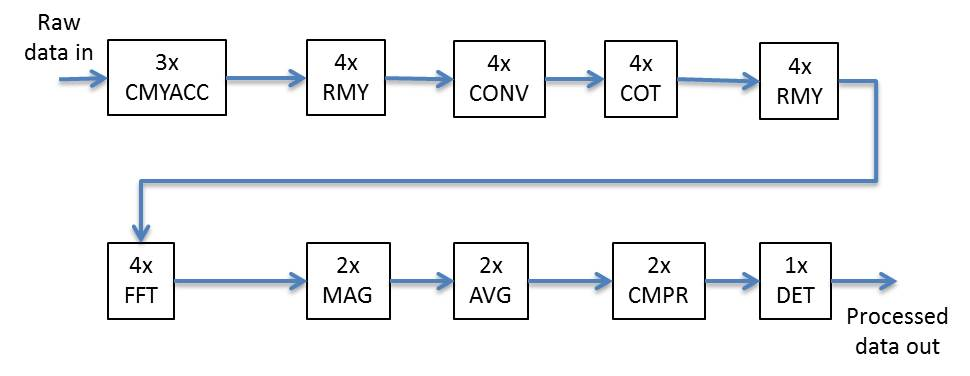
\includegraphics[width=160mm]{figures/aa_seq}
	\caption{A/A Mode, Sequence of Function Execution}
	\label{fig:bg_related_work:aa_seq}
\end{figure}
\FloatBarrier

\section{Design Decisions}
\label{mm:design_decisions}

\subsection{Parallel Execution}
Figure \ref{fig:mm:aa_serial_exe} illustrates the data distribution of Scheme-3 per CPU level. The diagram implies that the nature of execution is serial manner, in other words, it is equivalent to running the application on a single core processor. More CPUs and cores are used to improve the utilization factor, disregarding the processing time. Thumb rule to reduce the processing latency is to process data independent portions of the application in parallel. 

\begin{figure}[h!]
	\centering
	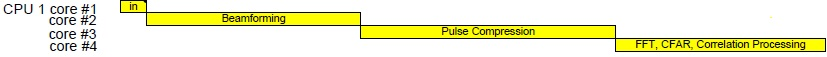
\includegraphics[width=160mm]{figures/aa_serial_exe}
	\caption{Serial Execution of A/A Mode Data in Existing Analysis}
	\label{fig:mm:aa_serial_exe}
\end{figure}

\subsection{Balanced Utilization}
In all the schemes of the Existing Analysis, core1 of A/A Mode CPU does only Input/Output operations, utilizing a smaller amount of the available CPU capability. Due to this, other cores of the CPU have to carry out rest of the processing, leaving them over utilized. This kind of skewed utilization figure pushes up the CPUs worst case utilization factor, so having well balanced load is a gesture of a healthy system. Core1 should also take part in processing the Radar application for load balancing as well as latency reduction. \vspace*{0.2cm}

\subsection{Space Partition}
Evaluating the results of Time Partition scheme against Space Partition scheme, former one is considered only to improve the utilization factors. Down sides of the Time Partition scheme are:
\begin{compactitem} 
\item It magnifies latency by 2x compared to the Space Partition scheme.
\item As it requires breaking the entire application to fit into time slot, it is not scalable (see Chapter \ref{sss:mm:cons:scalability}).
\item Implementation needs more attention when it comes to memory partitioning.
\item Failure of one CPU will affect both the A/A Mode and SAR Mode processing.
\end{compactitem} 
\vspace*{0.2cm}
To sum up, Time Partition demands more effort and time to realise but producing no better result than Space Partitioning. So, this thesis decides to choose Space Partition as a base for further mode mapping analysis.


\subsection{Dedicated Communication Channels}
Distributing the Radar raw data to different CPUs and gathering processed data increases total amount of communication. Dedicated channels for input, output between DGPM and PSM shall be established in Time Partition configuration. It facilitates receiving incoming data stream and sending out processed data simultaneously without interference. The DGPM has 6 ports Ethernet interface, of which 4 port shall be connected to 4 CPUs and remaining 2 ports shall act as dedicated input, output channels.

%%%%%%%%%%%%%%%%%%%%%%%%%%%%%%%%%%%%%
%%%%%%%%%%%%%%%%%%%%%%%%%%%%%%%%%%%%%
%%%%%%%%%%%%   SECTION   %%%%%%%%%%%%
%%%%%%%%%%%%%%%%%%%%%%%%%%%%%%%%%%%%%
%%%%%%%%%%%%%%%%%%%%%%%%%%%%%%%%%%%%%
\section{Scheme 4}
\label{sec:mm:scheme4}
According to the A/A Mode processing chain, only Correlation Processing is dependent on the previous 7 bursts. Rest of the processing steps do not have any dependency, thus can be performed independently. Final Correlation Processing shall be computed serially.

\subsection{Data distribution}
Each burst is distributed to different cores. Four core CPU gets four bursts to process till Thresholding and Detection stage. In the Figure \ref{fig:mm:scheme4_aa_mode_mapping}, CPU1...6 are allocated to processes 4 burst each and CPU7 does Correlation Processing.

\begin{tabular}{rl}
	No.of cores for burst processing: & 6 x 4 = 24 \\
	No.of cores for correlation processing: & 1 x 4 = 4 \\
	Data distribution-burst processing: & One burst per core \\
	Data distribution-correlation processing: & One dwell per core \\
\end{tabular}
%\FloatBarrier 


\begin{figure}[h!]
	\centering
	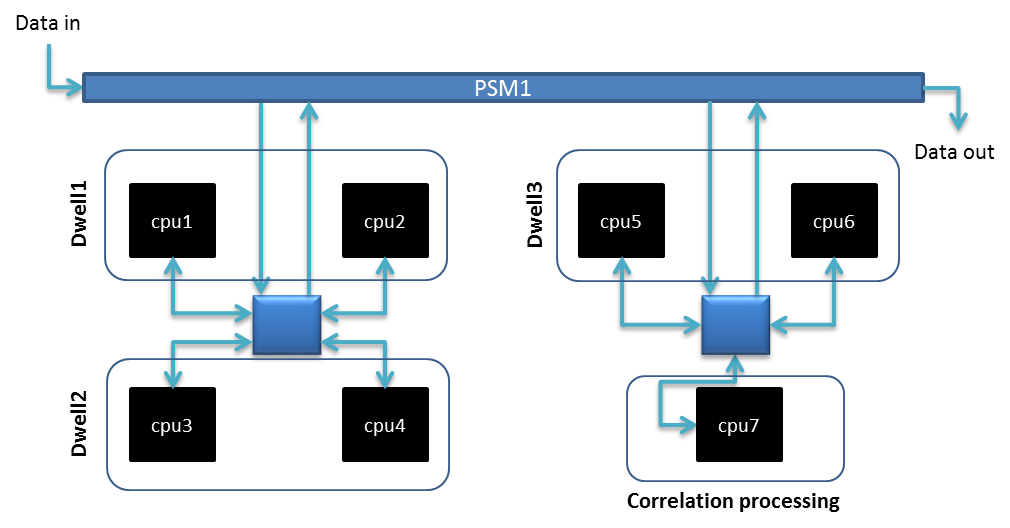
\includegraphics[width=160mm]{figures/scheme4_aa_mode_mapping}
	\caption{Scheme-4, Mode Mapping}
	\label{fig:mm:scheme4_aa_mode_mapping}
\end{figure}

The received A/A Mode raw data will be processed as follows

\begin{enumerate}
\item PSM1 routes each burst data to each core starting from core0 of CPU1 to core4 of CPU6 in round robin fashion.
\item Each core in the CPU1...6 performs Beamforming, Pulse Compression, FFT and CFAR processing followed by storing the results in SDRAM.
\item In a CPU, a core completing the processing steps last will transfer all the cores results to CPU7 for correlation processing. This avoids frequent communication between burst processing CPUs and correlation processing CPU. The data passed to the CPU7 is alarm list and their related information, which is smaller in size and assumed that it requires only 0.01ms to transfer.
\item Each core of the CPU7 waits for processed 8 burst data, and then performs Correlation Processing followed by sending out the target detections to PSM1.
\item PSM1 directs the results to tracking processor or display processor.
\end{enumerate}

\begin{figure}[h!]
	\centering
	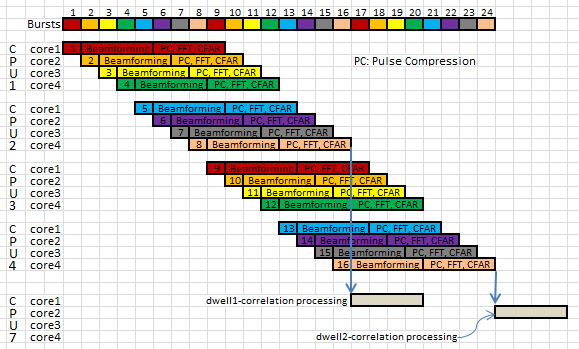
\includegraphics[]{figures/scheme4_data_distribution}
	\caption{Comparison of Data Distribution Schemes}
	\label{fig:mm:scheme4_data_distribution}
\end{figure}

\subsection{Hypothesis}
From the Figure \ref{fig:mm:scheme4_data_distribution}, Beamforming of the first burst will start only after receiving a complete dwell incase of existing analysis. Though the first burst is ready for Beamforming, redundant time is spent in waiting for the complete dwell data. This applies to the Pulse Compression, FFT, and CFAR processing also.\\[0.2cm]
Scheme-4 exploits the fact that every burst can be processed independently until the Thresholding and Detection stage. Every burst is sent to individual core to process them conveniently as soon as they are received. This saves waiting time during Data receive period, Beamforming, Pulse compression, FFT and CFAR processing. Nothing has changed in terms of Correlation Processing, hence it will not contribute to latency reduction.


\subsection{Processing Latency}
\label{ss:mm:scheme4:latency}
Processing latency is measured on a real hardware clocked 1GHz and the results are scaled down to 800MHz. Data transfer time of 0.02ms is assumed between CPU1...6 and CPU7. Total time required to process one burst until Thresholding and Detection stage is same as Scheme-1, the difference here is bursts are distributed over many cores. The \textsl{Sum of required time} values are different from Scheme-1 because the execution cycle of the benchmarks are evaluated and updated (see Chapter \ref{mm:cons:exe_cyl_mismatch}) as a contribution of this thesis. The stated values say that the look direction-1, PRF1 needs 35.72ms time to complete the execution from the moment a core starts receiving a burst. 

Elapsed wall clock time to process burst by burst is listed as \textsl{Time spent}. Example calculations for the look direction-1 are explained here. Cores wait for the pre-defined burst data to be received, i.e. a core processing PRF5 should wait till the PRF1...5 are distributed. Burst receive time are derived from the Radar characteristics (see Chapter \ref{ss:aa_mode:radar_char}).

\begin{figure}[h!]
	\centering
	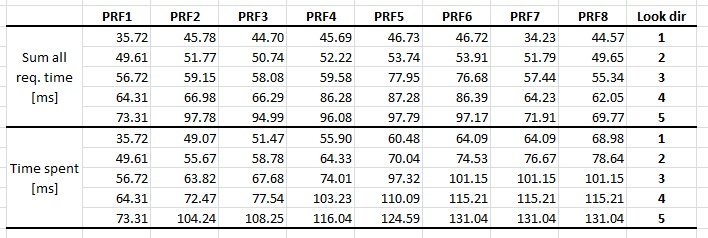
\includegraphics[width=140mm]{figures/scheme4_elapsed_time}
	\caption{Scheme-4, A/A Mode Processing Time}
	\label{fig:mm:scheme4_elapsed_time}
\end{figure}

\begin{align*}
	Elapsed \: time &= MAX((Previous \: burst \: receive \: time + Execution \: time), Elapsed \: time)\\
	PRF1 &= MAX((0 + 35.72), 0) = 35.72 \: ms\\
	PRF2 &= MAX((PRF1 \: receive \: time + Execution \: time), Elapsed \: time) \\
		&= MAX((3.28 + 45.78), 35.72) = 49.07 \: ms \\	 
	PRF3 &= MAX((PRF1...2 \: receive \: time + Execution \: time), Elapsed \: time) \\	
		&= MAX((3.28 + 3.50 + 44.7),49.07) = 51.47 \: ms \\
	PRF4 &= MAX((3.28 + 3.50 + 3.44 + 45.69), 51.47) = 55.90 \: ms \\
	PRF5 &= MAX((3.28 + 3.50 + 3.44 + 3.53 + 46.73), 55.90) = 60.48 \: ms \\
	PRF6 &= MAX((3.28 + 3.50 + 3.44 + 3.53 + 3.63 + 46.72), 60.48) = 64.09 \: ms \\ 
	PRF7 &= MAX((3.28 + 3.50 + 3.44 + 3.53 + 3.63 + 3.57 + 34.23), 64.09) = 64.09 \: ms \\	
	PRF8 &= MAX((3.28 + 3.50 + 3.44 + 3.53 + 3.63 + 3.57 + 3.46 + 44.57), 64.09) \\
		&= 68.98 \: ms	\stepcounter{equation}\tag{\theequation}
\end{align*}

Data transfer time of 0.02ms between burst processing CPUs and correlation processing CPU, and 0.2ms between correlation processing CPU and tracking/display processor is assumed.
\begin{align*}
	Latency &= Burst \: processing + Data \: transfer \: to \: CPU7 + Correlation \: processing \\
		& \qquad + Transfer \: results  \\
		&= 68.98 + 0.02 + 43.34 + 0.2 = 112.5 \: ms  \stepcounter{equation}\tag{\theequation}
\end{align*}
Data transfer time of 0.02ms between burst processing CPUs and correlation processing CPU, and 0.2ms between correlation processing CPU and tracking/display processor is assumed.
\begin{table}[h!]
	\centering
	\begin{tabular}{|c|l|l|l|} 
	 \hline
	 \textbf{Look direction} & \textbf{Dwell time[ms]} & \textbf{Latency[ms]} & \textbf{\#Dwell latency} \\
	 \hline
	 1 & 27.84 & 112.52 & 4.04 \\ \hline
	 2 & 33.07 & 122.18 & 3.69 \\ \hline
	 3 & 39.17 & 144.69 & 3.69 \\ \hline
	 4 & 46.20 & 158.75 & 3.44 \\ \hline
	 5 & 54.26 & 174.58 & 3.22 \\ \hline
	\end{tabular}
	\caption{Scheme-4, A/A Mode Processing Latency}
	\label{tbl:mm:scheme4_latency}
\end{table}

\subsection{CPU Load}
\label{ss:mm:scheme4:cpu_load}
CPU load is the ratio of processing time to the available time. 6 CPUs are involved in A/A Mode processing; meaning 24 cores are processing 3 dwell data. Available time is 3x dwell time. From the Figure \ref{fig:mm:scheme4_util}, maximum core utilization can reach up to 66\%. Calculations for the Look direction-1, PRF1 are explained here.
\begin{figure}[h!]
	\centering
	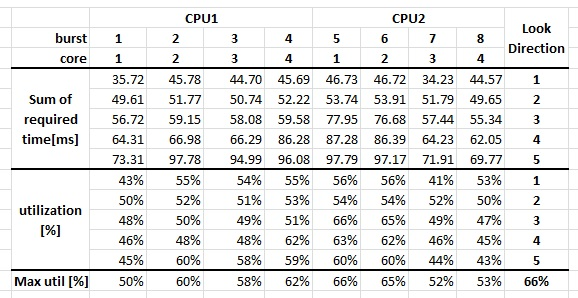
\includegraphics[width=140mm]{figures/scheme4_util}
	\caption{Scheme 4, A/A Mode CPU Utilization}
	\label{fig:mm:scheme4_util}
\end{figure}

\begin{align*}
	Required \: time &= 35.72 \: ms \\
	Available \: time &= 3 * dwell \: time = 3 * 27.84 = 82.2\: ms \\
	Utilization &= \frac{Required \: time}{Available \: time} = \frac{35.72}{82.2} = 43.4\% \stepcounter{equation}\tag{\theequation}
\end{align*}

\subsubsection{Utilization of Correlation Processing CPU}
\label{mm:SSS:scheme4:corr_cpu_util}
Updated correlation processing time values are listed in Figure \ref{fig:mm:scheme4_corr_calc}. Calculations are same as Scheme-1, the difference is operating system overhead factor is removed from the analysis.
\begin{figure}[h!]
	\centering
	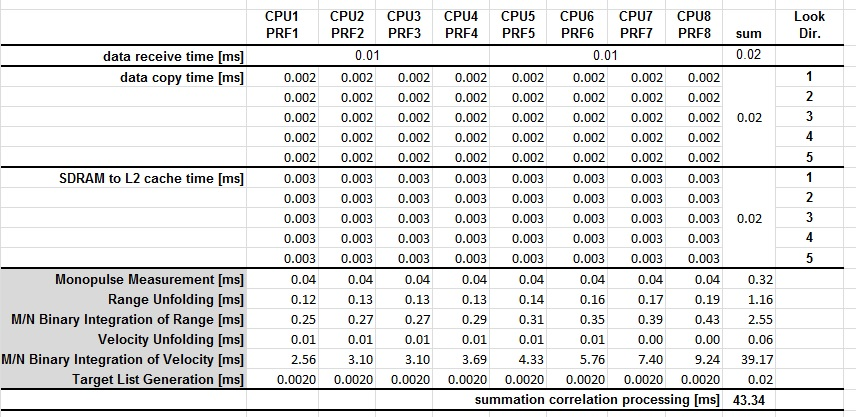
\includegraphics[width=160mm]{figures/scheme4_corr_proc}
	\caption{Scheme-4, Execution Time of Correlation Processing}
	\label{fig:mm:scheme4_corr_calc}
\end{figure}

Every core of the correlation processing CPU is in idle state until it receives processed one dwell data from CPU1...6. Then it continues processing for 43.34ms before returning to idle state. Dwells are distributed to 4 cores in round robin manner. From the Table \ref{tbl:mm:scheme4_corr_cpu_util}, peak utilization of the CPU7 is 39\%. 

Processed dwells are distributed to four cores of the CPU7 in cyclic scheme. Core1 of the CPU7 can start processing as soon as 8 bursts of a dwell are received. 1ms delay is assumed between burst processing CPUs sending out the data and CPU7 starts processing. From the Figure \ref{fig:mm:scheme4_elapsed_time}, look direction-1 needs 68.98ms to do burst processing. Until this time, CPU7 is in idle state. Correlation processing takes place for the next 43.34ms in core1 followed by waiting for the next set dwell5 data. Dwell5 will be supplied to the burst processing CPUs at 115.3ms (4 x 27.84ms) by the incoming stream. Received dwell5 data will be fed to CPU7 after 68.98ms (processing) + 1ms (transfer).

\begin{figure}[h!]
	\centering
	\includegraphics[width=160mm]{figures/scheme4_cor_cpu}
	\caption{Utilization of Correlation Processing CPU for Look direction-1}
	\label{fig:mm:scheme4_corr_cpu_util}
\end{figure}

\begin{align*}
	Utilization \: at \: dwell1 &= \frac{processing \: time}{processing \: time + waiting \: time } = \frac{43.34}{43.34 + 69.98} = 38\% \\[0.4cm]
	Next \: dwell \: time &= Dwell5 \: input \: at \: burst \: processing + Burst \: processing \: time \\
	&= 4 * 27.84 + 69.98 =181.3 \: ms\\
	Idle \: time &= Next \: dwell \: in - Last \: dwell \: out \\
	&= 181.33 - (69.98 + 43.34) = 68.01 \: ms \\
	Utilization \: at \: dwell5 &= 	\frac{43.34}{43.34 + 68.01} = 39\%  \stepcounter{equation}\tag{\theequation}
\end{align*}

\begin{table}[h!]
	\centering
	\begin{tabular}{|c|l|} 
	 \hline
	 \textbf{Look direction} & \textbf{Max CPU Utilization} \\
	 \hline
	 1 & 39\%  \\ \hline
	 2 & 35\%  \\ \hline
	 3 & 30\%  \\ \hline
	 4 & 27\%  \\ \hline
	 5 & 25\%  \\ \hline
	\end{tabular}
	\caption{Utilization of Correlation Processing CPU}
	\label{tbl:mm:scheme4_corr_cpu_util}
\end{table}
Utilization drops for ascending look direction, since look direction 5 has longest data receive time and processing time but maximum target detections are same for all the look directions. Utilization calculation and worst case utilization for look direction-1, core1 is given below. 

\subsection{Memory Utilization}
\label{ss:mm:scheme4:mem_util}
From the \verb|mem_util.sh| script, it is measured that the Radar application is consuming only 1.0\% of the available 879MiB memory.

\subsection{Memory Transfer Bandwidth}
\label{ss:mm:scheme4:bw_util}
Peak memory transfer bandwidth is measured as 41\% of the available 1048MiB/s.

\subsection{Summary}
\label{ss:mm:scheme4:summary}
Scheme-4 has 4 dwell time latency, 66\% CPU utilization, 41\% memory transfer bandwidth utilization and 1\% memory utilization. CPU utilization can be improved by simply adding more DGPMs. A comparison of Scheme-1, Acceptable values and Scheme-4 is given below.

\begin{table}[h!]
	\centering
	\begin{tabular}{|l|l|l|l|} 
	 \hline
	 \textbf{Parameter} & \textbf{Scheme-1} & \textbf{Acceptable Values} & \textbf{Scheme-4}\\
	 \hline
	 Dwell latency &  14.96 & 2 & 4.04 \\ \hline
	 CPU load & 75.5\% & \textless 50\% & 66\% \\ \hline
	 Memory Utilization & 7\% & \textless 50\%  & 1\% \\ \hline
	 Memory transfer bandwidth & NA & \textless 50\% & 41\%  \\ \hline
	\end{tabular}
	\caption{Comparison of Scheme-1 vs Acceptable Values vs Scheme-4}
	\label{tbl:mm:scheme4_comparison}
\end{table}


%%%%%%%%%%%%%%%%%%%%%%%%%%%%%%%%%%%%%
%%%%%%%%%%%%%%%%%%%%%%%%%%%%%%%%%%%%%
%%%%%%%%%%%%   SECTION   %%%%%%%%%%%%
%%%%%%%%%%%%%%%%%%%%%%%%%%%%%%%%%%%%%
%%%%%%%%%%%%%%%%%%%%%%%%%%%%%%%%%%%%%
\section{Scheme 5}
\label{sec:mm:scheme5}

\subsection{Hypothesis}
\begin{compactitem}

\item Taking a closer look into the processing chain in Chapter \ref{sec:bg_related_work:proc_chain}, revels that a burst data has 4 channel processing namely Sum, Guard, Azimuth and Elevation.  These 4 channels do not have data dependency, allowing for parallel execution. Figure \ref{fig:mm:scheme5_data_path}, shows the data dependency diagram for A/A Mode processing.

\begin{figure}[h!]
	\centering
	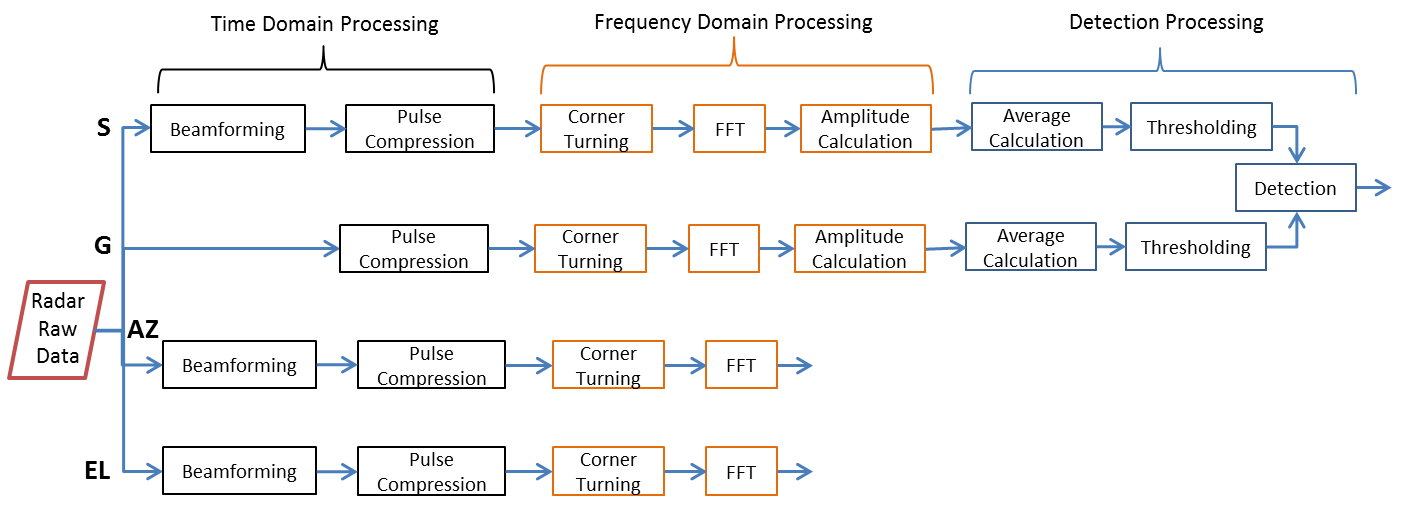
\includegraphics[width=160mm]{figures/scheme5_data_path}
	\caption{A/A Mode Data Dependency of Benchmarks}
	\label{fig:mm:scheme5_data_path}
\end{figure}
Note: The data dependency diagram doesn't consider constant table values, as they are pre-calculated and available at any point of time.

\item Correlation processing shall be optimized to bring down the execution time.
\end{compactitem}

\subsection{Data Distribution}
\label{ss:mm:scheme5:data_distribution}
Four channel processing are done by 4 cores of a CPU. CPU1...12 gets one burst each. CPU13 and CPU14 are allocated for correlation processing. 
PSM1 routs the Radar raw data to the respective DGPMs. Processed burst data are sent to PSM1 by CPUs. PSM stores the burst result until 8 burst results are received. Then 8 burst results are sent to the cores of CPU13,14 in round robin manner. 

In terms of burst processing, every CPU in Scheme-4 performs computation on 4 burst data, whereas a CPU in Scheme-5 does computations on one burst. Single burst is placed in shared memory, so that all the four cores can access them. This analogy applies to the correlation processing CPUs also. Any correlation processing CPU in Scheme-5 processes one dwell data, on contrary to the 4 dwell data in Scheme-4. It results in 4x reduced memory requirement than Scheme-4.

\begin{figure}[h!]
	\centering
	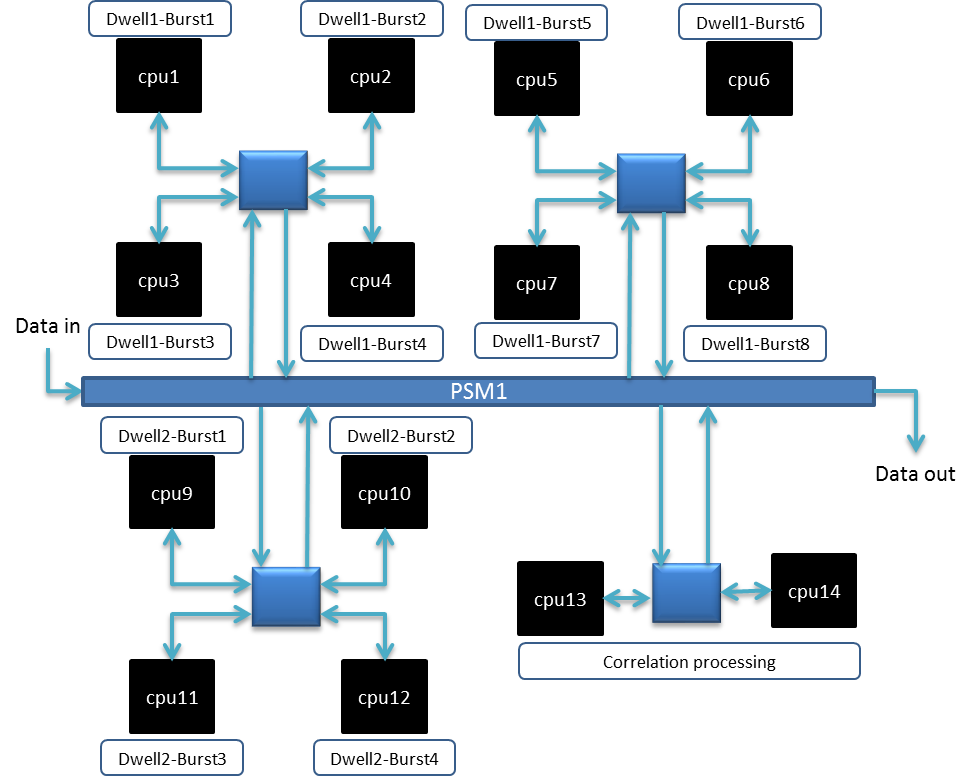
\includegraphics[width=160mm]{figures/scheme5_mode_mapping}
	\caption{Scheme-5, Mode Mapping}
	\label{fig:mm:scheme5_mode_mapping}
\end{figure}

Correlation processing requires 43.34ms (see Chapter \ref{mm:SSS:scheme4:corr_cpu_util}) to process one dwell data. Dwell time of look direction-1 is 27.84ms. Correlation processing itself consumes 1.5x dwell time. Best result cannot be achieved without optimizing the correlation processing. According to the derivations of measurement time, M/N Binary Integration of Velocity consumes 39.16ms of total 43.34ms. It is a good candidate for optimization. M/N Binary Integration of Velocity is implemented in \verb|C| program and the execution time is measured as 31.52ms. Loop iteration data are independent and they are broken in to four loops running on four cores of a CPU. 4x speedup is achieved for M/N Binary Integration of Velocity. Resulting processing time is reduced to 7.88ms. Correlation processing all together needs 12.06ms time to process one dwell.

\begin{figure}[h!]
	\centering
	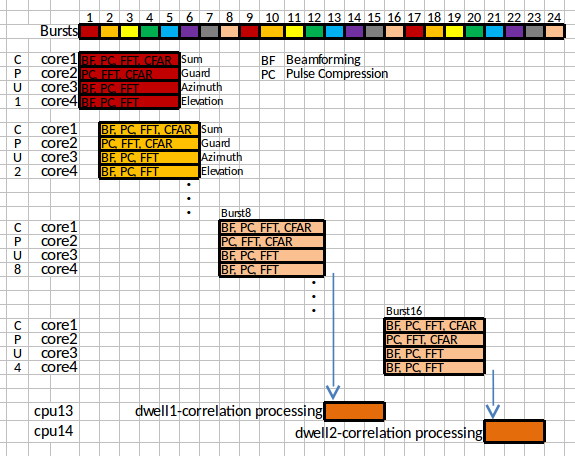
\includegraphics[]{figures/scheme5_data_distri}
	\caption{Scheme-5 Data Distribution}
	\label{fig:mm:scheme5_data_distri}
\end{figure}


\subsection{CPU Load}
\label{ss:mm:scheme5:cpu_load}
Twelve CPUs are processing one burst each. Available time of a CPU is the time span between reception of two bursts to the CPU, which is 12x average burst time. From the following figures, it is implied that the peak CPU utilization reaches up to 50.8\%. Look direction-2 to 4 are not shown in the figures for simplicity, anyway look direction-5 contributes to the worst case.

\begin{figure}[h!]
	\centering
	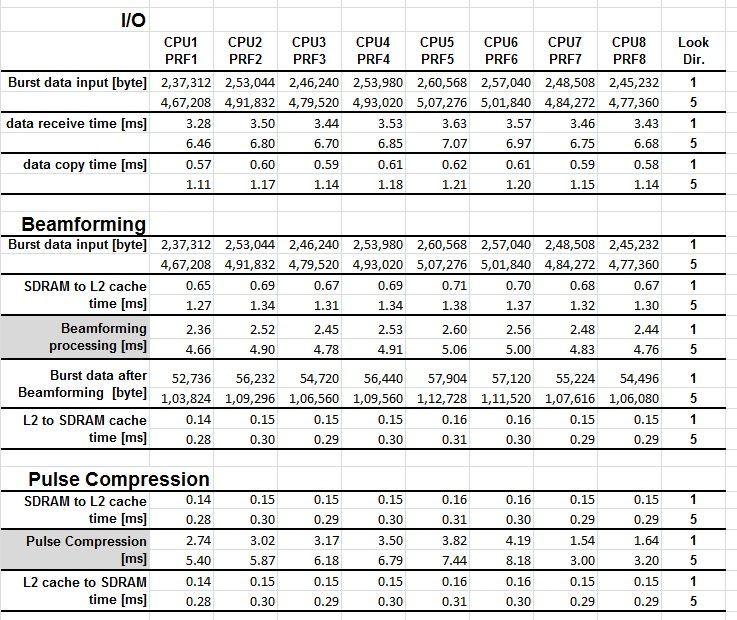
\includegraphics[width=160mm]{figures/scheme5_cpu_util1}
	\caption{Scheme-5, CPU Utilization (1/2)}
	\label{fig:mm:scheme5_cpu_util1}
\end{figure}
Nothing has changed in I/O processing and Burst data input of the Beamforming. CPU time spent on processing is explained for PRF1, look direction-1. Listed calculations illustrate one channel processing per core, comprises of executing maximum 10 benchmarks. Reaming cores of the CPU executes the same benchmark in parallel or skips to the next benchmark, meaning that when one core completes complex multiply algorithm, other cores also would have completed. This is confirmed by measuring the worst case execution time of the Scheme-5 implementation.

\begin{align*}
\label{aa:scheme5:equ1}
	SDRAM \: to \: L2cache &= 237,312 byte \, * \, 2.18\frac{cycle}{byte} \, * \, 1.25\frac{ns}{cycle} = 0.65 \: ms \\[0.3cm]
	Beamforming &= 1channel * 64pulses * 103 \frac{range gates}{pulse} * 287\frac{cycle}{8 element} \\[0.3cm] 
	&\qquad * 1.25\frac{ns}{cycle} = 2.36 \: ms\\[0.3cm]
	Beamformed \: data &= 1channel * 64pulses * 103 \frac{range gates}{pulse} *8\frac{byte}{sample} = 52,736 \: byte \\[0.3cm]
	L2cache \: to \: SDRAM &= 52,736 byte \, * \, 2.18\frac{cycle}{byte} \, * \, 1.25\frac{ns}{cycle} = 0.14 \: ms \\
	Pulse \: compression &= \bigg(\#channel * \#pulses (CONV128 +  \# \frac{range gates}{pulse} * RMY50)\bigg) \\
			& \quad * cycle \: time \\
			&= (1 * 64 (27300 + 103 * 68)) * 1.25ns = 2.74 \: ms \stepcounter{equation}\tag{\theequation} 
\end{align*}

\begin{figure}[h!]
	\centering
	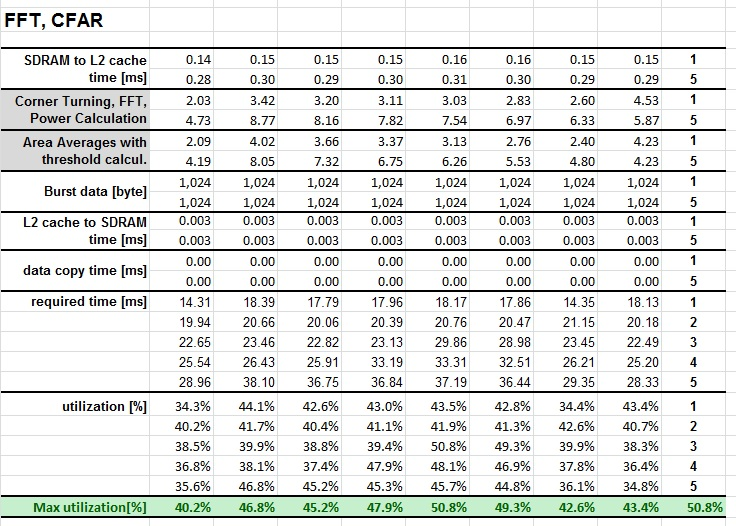
\includegraphics[width=160mm]{figures/scheme5_cpu_util2}
	\caption{Scheme-5, CPU Utilization (2/2)}
	\label{fig:mm:scheme5_cpu_util2}
\end{figure}

\begin{align*}
	FDP \: time &= \bigg(1channel * (\#pulses * \# \frac{RG}{pulse} (COT50 + RMY50) + \# \frac{RG}{pulse} * \\
		& \qquad FFT64) + 1 * (\# \frac{range gates}{pulse} * 64 * MAG256)\bigg) * cycle \, time \\[0.3cm]
		&= (1 * (64 * 103 (98 + 68) + 103 * 2550) + 1 * (103 * 64 * 41)) * 1.25ns \\
		&= \enspace 2.03 \: ms \\
		Average \: Calculation &= 1channel * 103 \frac{range gates}{pulse} * 64(FFTsize) * 51(AVG100) * 2 \\
		&=  672,384 \: cycle \\
		Thresholding &= 1channel * 103 \frac{range gates}{pulse} * 64(FFTsize) * 55(CMPR100) \\
		&= 362,560 \: cycle \\
		Detection &= 103 \frac{range gates}{pulse} * 64(FFTsize) * 97(DET100) = 639,424 \: cycle \\
		Sum \: time &= (Average \: calculation + Thresholding + Detection) * cycle \: time \\
		&= (672,384 + 362,560 + 639,424) * 1.25ns = 2.09 \: ms	\stepcounter{equation}\tag{\theequation} 
\end{align*}

Total time required to process one burst by a core is calculated as the sum of IO processing, Beamforming, Pulse compression, FFT, CFAR, Thresholding, Detection and data copy time between SDRAM to the core. CPU utilization is the ratio of processing time to the available time. Calculations for the look direction-1, CPU1 is explained here.

\begin{align*}
	Available \: time &= \#CPUs * Avg. \: burst \: time = 12 * \frac{27.84ms (dwell \: time)}{8(\#burst)} = 41.76 \: ms\\[0.3cm]
	CPU \: utilization &= \frac{processing \: time}{available \: time} = \frac{14.31}{41.76} = 34.3\% \stepcounter{equation}\tag{\theequation} 
\end{align*}


\subsubsection{Correlation Processing} 
The data processed by the CPU1...10 are grouped as dwells and sent to CPU11 and CPU12 alternatively. Correlation processing CPUs are in idle state until they receive a dwell data then performs computation for 12.06ms followed by waiting for next set of dwell. 0.02ms time delay between burst processing CPUs and correlation processing CPUs is assumed. Utilization calculations for the look direction-1 are listed below. 

\begin{figure}[h!]
	\centering
	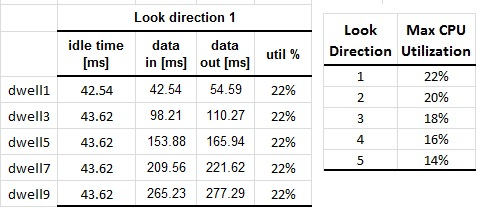
\includegraphics[]{figures/scheme5_mul_cpu_util}
	\caption{Scheme 5, A/A Mode Correlation Processing CPU Utilization}
	\label{fig:mm:scheme5_mul_cpu_util}
\end{figure}

\begin{align*}
	Utilization \: at \: dwell1 &= \frac{processing \: time}{processing \: time + waiting \: time } = \frac{12.06}{12.06 + 42.54} = 22\% \\[0.4cm]
	Next \: dwell \: time &= Dwell3 \: input \: at \: burst \: processing + Burst \: processing \: time \\
	&= 2 * 27.84 + 42.54 = 98.2 \: ms\\
	Idle \: time &= Next \: dwell \: in - Last \: dwell \: out \\
	&= 98.2 - (12.06 + 42.54) = 43.6 \: ms \\
	Utilization \: at \: dwell3 &=  \frac{12.06}{12.06 + 43.6} = 22\%  \stepcounter{equation}\tag{\theequation}
\end{align*}
From the Figure \ref{fig:mm:scheme5_mul_cpu_util}, peak utilization of the correlation processing CPUs reaches upto 22\% when using two CPUs. 

\subsection{Processing Latency}
\label{ss:mm:scheme5:latency}
Processing latency between 54.79ms and 88.17ms is achieved depending on the look direction, which is the time required for burst processing and correlation processing. Maximum dwell latency is 1.97x dwell time contributed by the look direction-1.

\begin{table}[h!]
	\centering
	\begin{tabular}{|c|l|l|l|} 
	 \hline
	 \textbf{Look direction} & \textbf{Dwell time[ms]} & \textbf{Latency[ms]} & \textbf{\#Dwell latency} \\
	 \hline
	 1 & 27.84 & 54.79 & 1.97 \\ \hline
	 2 & 33.07 & 61.43 & 1.86 \\ \hline
	 3 & 39.17 & 69.10 & 1.76 \\ \hline
	 4 & 46.20 & 77.98 & 1.69 \\ \hline
	 5 & 54.26 & 88.17 & 1.62 \\ \hline
	\end{tabular}
	\caption{Scheme-5, A/A Mode Processing Latency}
	\label{tbl:mm:scheme5_latency}
\end{table}

\subsection{Memory Utilization}
\label{ss:mm:scheme5:mem_util}
From the \verb|mem_util.sh| script, it is measured that the Radar application is consuming only 0.5\% of the available 879MiB memory. Memory requirement is reduced since, One CPU is working on one burst data. Whereas in Scheme-4, one CPU gets 4 burst data. 

\subsection{Memory Transfer Bandwidth}
\label{ss:mm:scheme5:bw_util}
Memory footprint is reduced compared to Scheme-4, leading to smaller operating data set per core. Private L1 cache and shared L2 cache can hold large portion of the operating data set, reducing memory transfer between SDRAM to core and so reducing memory transfer bandwidth. Peak memory transfer bandwidth is measured as 30\% of the available 1048MiB/s.

\subsection{Summary}
\label{ss:mm:scheme5:summary}

Processing latency of 1.92x dwell time and peak CPU utilization of 50.8\% are healthy values for Air to Air Mode Radar processor. It has remaining 49\% of the CPU utilization to accommodate future development. In fact, 8 CPUs are sufficient to give same processing latency. More CPUs are used to improve the utilization. Figure \ref{fig:mm:scheme5_summary} shows the relationship between number of CPUs used and their utilization without affecting the latency values. Any combination of the CPU sets can be chosen to achieve desired CPU load. A comparison of  Scheme-1, Acceptable values and Scheme-5 is given below.

\begin{figure}[h!]
	\centering
	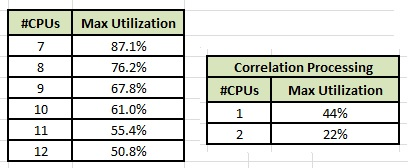
\includegraphics[]{figures/scheme5_summary}
	\caption{Scheme 5, Relationship Between Number of CPUs and Utilization}
	\label{fig:mm:scheme5_summary}
\end{figure}

\begin{table}[h!]
	\centering
	\begin{tabular}{|l|l|l|l|} 
	 \hline
	 \textbf{Parameter} & \textbf{Scheme-1} & \textbf{Acceptable Values} & \textbf{Scheme-5}\\
	 \hline
	 Dwell latency &  14.96 & 2 & 1.97 \\ \hline
	 CPU load & 75.5\% & \textless 50\% & 50.8\% \\ \hline
	 Memory Utilization & 7\% & \textless 50\%  & 0.5\% \\ \hline
	 Memory transfer bandwidth & NA & \textless 50\% & 30\%  \\ \hline
	\end{tabular}
	\caption{Comparison of Scheme-1 vs Acceptable Values vs Scheme-5}
	\label{tbl:mm:scheme5_comparison}
\end{table}

\section{Overview}
The Existing Analysis has been observed to spot the latency contributors, bottlenecks and data dependencies. Upsides and downsides are evaluated to bring up a best mode mapping scheme. Examined information have supported in design decisions of the mode mapping. Two new schemes are proposed to reduce the processing latency and they are validated via implementation.

Scheme-4 makes use of the fact that, the bursts in a dwell can be processed independently until Thresholding and Detection stage. This phenomenon skips waiting time in Beamforming, Pulse compression, FFT, CFAR, Thresholding and Detection stage. This can be called as coarse grained parallelism. A dedicated processor is assigned for Correlation processing, without changing the execution method. Final outcome of the Scheme-4 is 4x dwell latency with 66\% CPU utilization.

Every burst data has large amount of fine grained parallelism. Four channel processing of a burst is done independently in Scheme-5, saving the waiting time for the other channel processing.  Correlation processing poses a bottleneck as the serial execution requires 1.5x dwell time. Further, it is also parallelised and executed in dedicated CPUs. Deemed 2x processing latency is achieved along with 50.8\% CPU utilization, provided 13 CPUs are performing computation. Speedup of the Scheme-5 compared to the best scheme(Scheme-1) in the Existing Analysis is drawn below.

\begin{figure}[h!]
\centering
	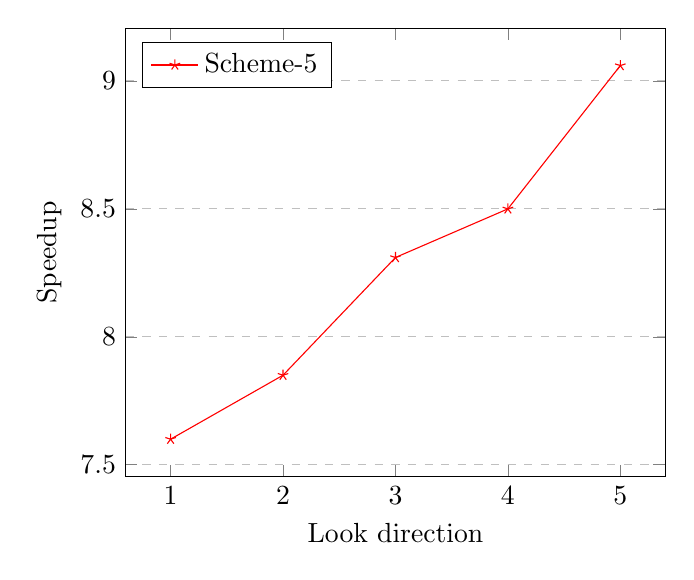
\begin{tikzpicture}
		\begin{axis}[
			xlabel={Look direction},
			ylabel={Speedup},
			legend pos=north west,
			ymajorgrids=true,
			grid style=dashed,
		]
		\addplot[color=red, mark=star,]
			coordinates {
				(1, 7.6) (2, 7.85) (3, 8.31) (4, 8.50) (5, 9.06)
			};
		\legend{Scheme-5}
	\end{axis}
\end{tikzpicture}
\caption{Speedup, Scheme-5 vs Scheme-1}
\label{mm:scheme5_speedup}
\end{figure}
